\chapter{Teoretická část}\label{resere}
TODO reserse neni dokoncena
\section{Pravidla farameworku Angular pro Git}\label{reserse:git}
    Na začátku je potřeba říct, že framework Angular není využít v této bakalářské práci. Prozkoumané pravidla nebyly kompletně převzaty. Byla provedena analýza a následně byly převzata část, která
    je použitelná při implementaci serveru, který je předmětem teto bakalářské práci. Kompletní přehled pravidel se nachází na GitHub\footnote{ GitHub je webový platformou pro vývoj softwaru pomocí systému řízení verzí Git}\cite{angular-git}.
    
    Pravidla, které byly použity v této bakalářské práce, definují formátování pro \verb|commit| v rámci verbovacího systému Git\footnote{TODO git}. Příčinou zavedení konvenci je potřebnost přidání přehledností dřevu větví. Po dokončeni této bakalářské práci, server bude kompletně funkční, ale proces vývoje se tím neskončí. Budoucí kroky budou podrobně popsány v kapitole \ref{zhodnocení} . Pochopení jednotlivým změnám během vývoje softwaru pomáhají srozumitelné popisy jednotlivých změn. Dosažení takového výsledku působí zavedení jednoho formátu pro každý \verb|commit| v rámci projektu.
    
    \begin{figure}
            \begin{minted}{text}
<type>(<scope>): <subject>
<BLANK LINE>
<body>
<BLANK LINE>
<footer>
            \end{minted}
            \caption{Formát pro \texttt{commit} podle pravidel definovaných pro framework Angular} 
            \label{code:angular-commit}
    \end{figure}
    \begin{figure}
	   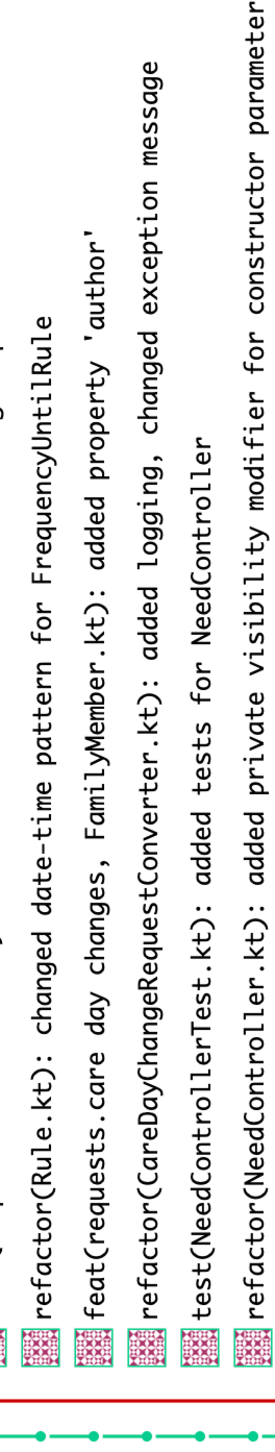
\includegraphics[angle=-90, width=1.0\textwidth]{pdfs/GitLabTree}
	   \caption[Ukázka použití konvenci pro práci z Git]{Ukázka použití konvenci pro práci z Git na grafu větví} 
    \end{figure}
    Tato konvence byla zavedena v moment začátku práci autora na implementaci bakalářské práci (viz obrázek \ref{image:gitlab-tree}). Struktura pro \verb|commit|, která je definovaná ve zbroji (viz obrázek \ref{code:angular-commit}), se skládá z šestí častí, které byly kompletně převzaty nebo upraveny:
    \begin{itemize}
        \item \texttt{type}
        \item \texttt{scope}
        \item \texttt{subject}
        \item \texttt{body}
        \item \texttt{footer}
    \end{itemize}
    
    \subsection{Type}
        Typ definuje část aplikace, které udělaný \verb|commit| mění. Seznám hodnot, které je možné zadat, je omezený předem definovaným seznamem:
        \begin{itemize}
            \item \texttt{build} -- změny procesu sestavení aplikace nebo úpravy externích závislostí
            \item \texttt{ci} -- změny tykající průběžné integrace
            \item \texttt{docs} -- změny tykající se jenom dokumentace
            \item \texttt{feta} -- přidání nových funkcí
            \item \texttt{fix} -- oprava chyb
            \item \texttt{perf} -- změny zvyšující efektivitu
            \item \texttt{refactor} -- změny, které nepřidávají nové funkcí a současně neopravují chyby
            \item \texttt{style} -- změny, které nemění význam kódu
            \item \texttt{test} -- přidaní nebo úprava testů
        \end{itemize}
    
    \subsection{Scope}
        Rozsah definuje konkretní soubory nebo baličky, které byly změněny. Rozsah není povinným, ale v rámci této bakalářské práci bude uveden pro každý \verb|commit|. V případě, že změny současně udělaný v několika různých souborech nebo balíčcích, je potřeba uvést je jako seznám oddělaný čárkami v kulatých závorkách.
    
    \subsection{Subject}
        Předmět je stručným popisem udělaných změn. Změny mají být odděleny od typu dvojtečkou. V případě, že \verb|commit| obsahuje několik změn, je potřeba je oddělit čárkou. První písmeno každé změny musí být malé. Poslední změna nekončí tečkou.
    
    \subsection{Body}
        Tělo je určeno pro podrobnější popis udělaných změn. Táto část není povinná, ale je doporučena v případě, že udělané není srozumitelné po stručném popisu v předmětu nebo není jasná příčina udělané změny.
    
    \subsection{Footer}
        Zápatí je určeno pro definování přelomových změn a definování závislostí na konkretní požadavky v rámci GitHub nebo GitLab\footnote{TODO GitLab}. V rámci této bakalářské práci každému požadavku v rámci GitLab jsou přiděleny jednotlivé větví, proto není potřeba uvádět identifikátor požadavku ve zápatí.
    
\section{Kotlin}\label{resere:kotlin}
    Kotlin je relativně nový jazyk pro JVM\footnote{Java Virtual Machine}. Poprvé tento jazyk byl představen společnosti v 2011 roku. První stabilní verze byla představena v únoru roku 2016. Ale už v květnu roku 2017 Kotlin se stal oficiálním jazykem pro Android.
    
    Kotlin byl vytvořen jako alternativa jazyku Java a řeší některé jí problémy. Například, Kotlin řeší problém použití null, také známý jako \textit{The Billion Dollar Mistake}\cite{theBDM}, a spojené s ní problémy. Java samotna nemá podporu pro \textit{not-null} proměnné, ale Kotlin takovou podporu má, a to v podobě oddělení \textit{nullable} typu pomocí ? operátoru.
    
    Kotlin je odlišný od Javy i syntaxí. Například není potřeba psát středník pro dokončeni příkazu, ale je vyžadován pouze v případe, že chcete oddělit několik příkazů na jedné řádce. Také byly odstraněny spousta klíčových slov. Například pro deklarací \textit{public final} proměnné je potřeba použit klíčově slovo \textit{val}. Důležitým rozdílem je, že při vytvoření třídy Kotlin umí vygenerovat metody \textit{get} a popřípadě i \textit{set} a umožňuje zadávat defaultní hodnoty v konstruktoru. Také Kotlin zavádí \textit{data class}, který navíc od obyčejné třídy umí vygenerovat metod \textit{toString}, který převádí třídu na typ \textit{String} v čítelné podobě \cite{Priklad vygenerovane tridy}, a metody \textit{equals} a \textit{hashCode}. Celý seznam věcí, které Kotlin má navíc od Javy nebo má jinou implementaci, což není předmětem teto práci, nemá smysl. Proto 
    
    
    Kotlin je Kotlin podporuje \textit{type-safe builder}
\section{Spring}\label{resere:j2ee}
    
\section{Testování}\label{resere:testovani}
    \subsection{Spring}
    TODO popis nastroju pro testovani
    \subsection{JUint 5}
    TODO popis nastroju pro testovani
    \subsection{JaCoCo}\label{resere:testovani:jacoco}
    TODO nastroj pro analyzu pokryti kodu testy \cite{JoCoCo}
    \subsection{IntelliJ IDEA}\label{resere:testovani:intellij-idea}
    TODO nastroj pro analyzu pokryti kodu testy \cite{intellij-idea-code-coverage}

\section{Dokumentace}\label{resere:dokumentace}
    Swagger
    
\section{Databáze}\label{resere:databaze}

    \subsection{H2}
        TODO Pro proces vývoje a testování byla zvolena databáze H2\cite{h2-db}, která je relační databází. 
    \subsection{PostgresSQL}
        TODO PostgresSQL
    
\section{Buildováci sstém}\label{resere:build}
    TODO Gradle...

\section{CLOC}\label{reserse:cloc}
    Nástroj CLOC\footnote{Count Lines of Code}\cite{cloc-download} poskytuje možnost spočítat počet řádek kódu v dáne složce. Nástroj podporuje velký počet jazyku programování. Výsledek obsahuje počet řádek kódu oddělený od komentářů a prázdných řádků.